\chapter[Results]{Results} \label{ch:results}

Here we present the results of our primary and alternative optimization strategies.
All random circuits are generated using the \codeword{CNOT_HAD_PHASE_circuit} method in PyZX which constructs a circuit consisting of CNOT, HAD, and phase gates.
Default parameters are used for the probability of each gate type.

\section{Primary Strategy}

Before reporting on the results of our primary optimization strategy, we first conduct preliminary analyses to refine our method.
After finalizing these refinements, we report on the performance of this strategy.

\subsection{Refinements}

The opportunities for refinement are the following:
\begin{itemize}
\item
  Optimization function
\item
  Probability of applying Equation \ref{eq:gen-io-lc} vs. Equation \ref{eq:gen-io-pivot}
\item
  Sampling of subjects (i.e., spiders or pairs of connected spiders) for congruence application
% \item
  % Probability of applying \codeword{full_reduce} throughout search, $p_{fr}$ % FIXME: Could just skip this one...
\end{itemize}
For these analyses, we only use SA as it is more computationally efficient and we expect the behavior of these refinements to generalize to GA.

\subsubsection*{Optimization Function}

First, we test if any property of a ZX-diagram could serve as a reliable proxy for the complexity of its associated circuit.
To do so, we first generated 500 random circuits (10 qubits, 100 gates) and immediately converted them to ZX-diagrams.
Given this library of ZX-diagrams, we then measured the Pearson correlation coefficient between the complexity of the extracted circuit and each ZX-diagrammatic property discussed in Section \ref{sec:obj-funcs}.
The following table summarizes these correlations:
\begin{center}
% \begin{table*}[h!]
\begin{tabular}[]{@{}lcc@{}}
\toprule
                    & $r$ & p-value \\ \midrule
\# Edges  & 0.097        & 0.029            \\
Centrality & 0.090        & 0.045            \\
Density    & -0.096       & 0.032            \\ \bottomrule
\end{tabular}
% \caption{\label{tab:obj-pearson}Correlations between various ZX-diagrammatic properties and the complexity of the extracted circuit for 500 randomly generated ZX-diagrams. Pearson's correlation coefficient is denoted $r$ and the 2-tailed p-value is provided. The ZX-diagrams were generated by converting 500 random circuits with 10 qubits and 100 gates to ZX-diagrams.}
% Table \ref{tab:obj-pearson} summarizes these correlations.
% \end{table*}
\end{center}
Pearson's correlation coefficient is denoted $r$ and the 2-tailed p-value is provided.
From these data, it is clear that no identified property of a ZX-diagram can serve as a reliable proxy for the complexity of its associated circuit.
Therefore, the default scoring method discussed in Section \ref{sec:primary} that relies on extraction is used for the remainder of our analyses.



\begin{figure}[t]
\centering
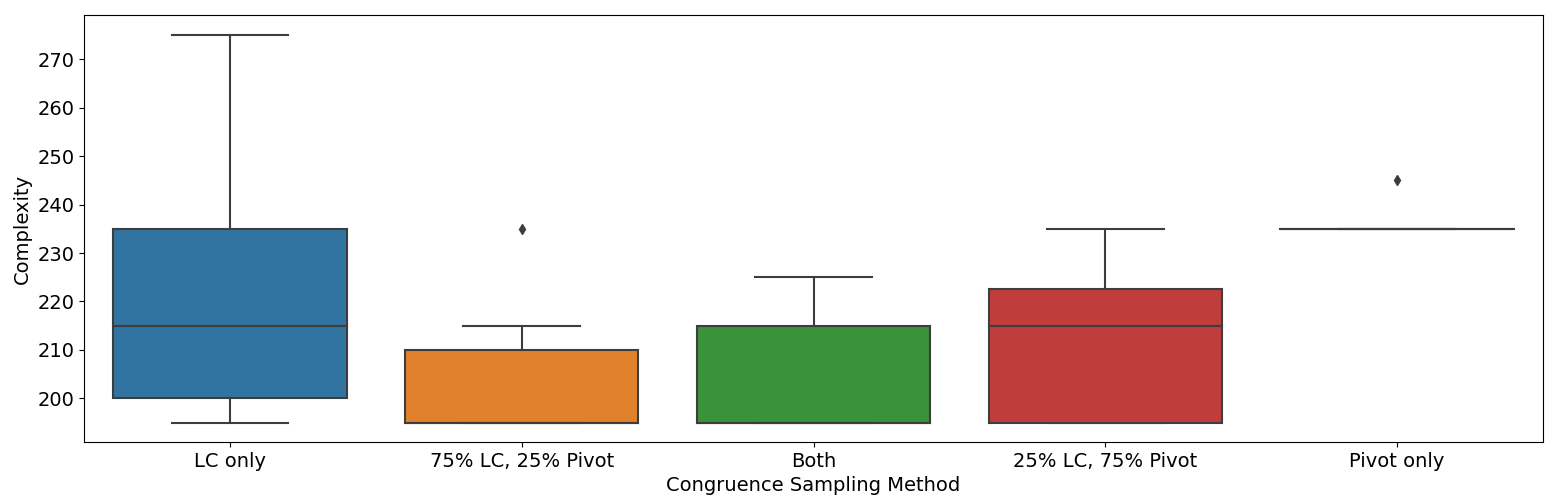
\includegraphics[width=13cm]{img/cong-sampling-ex.png}
\caption{
  A representative comparison of congruence sampling methods for a 5 qubit, 50 gate circuit.
  All three sampling methods that include both LC and pivoting achieve the best simplification in the alotted number of steps.
  When using only local complementation (i.e., Equation \ref{eq:gen-io-lc}), the same best-case complexity is achieved over the 10 trials but the average complexity is higher.
  Alternatively, using only pivoting does not achieve the same reduced circuit.
}
\label{fig:cong-sampling}
\end{figure}

\subsubsection*{Congruence Sampling}

By default, we apply Equations \ref{eq:gen-io-lc} and \ref{eq:gen-io-pivot} with equal probability ($p_{LC} = p_{pivot} = 0.5$).
However, it may be the case that one congruence should be chosen more frequently than the other.
To evaluate this, we generated 30 random circuits (5 qubits, 50 gates) and repeated search with a range of $(p_{LC}, p_{pivot})$ pairs.
For a given circuit, search was performed 10 times for each pair and the complexities of the optimized circuits were plotted according to congruence sampling probabilities.
In all cases, the sampling methods that include both LC and pivoting yielded the lowest average complexity across the 10 trials as well as the least complex circuit overall.
% In some cases, other sampling methods matched, but never outperformed this method in either metric.
There were no significant differences between the three combined sampling methods (i.e., 50/50, 25/75, and 75/25) and the LC- ($p_{LC} = 1.0$, $p_{pivot} = 0.0$) or pivot-only ($p_{LC} = 0.0$, $p_{pivot} = 1.0$) sampling methods sometimes matched, but never outperformed these combined methods.
% Most notably, the least cusing only local complementation (i.e., $p_{LC} = 1.0$, $p_{pivot} = 0.0$) produced a circuit that matched the
Most notably, the least complex circuit identified using LC-only matched the minimum complexity 73.3\% of the time while that identified using pivot-only was more complex than the best-case 86.7\% of the time.
% Most notably, the least complex circuit identified using only local complementation (i.e., $p_{LC} = 1.0$, $p_{pivot} = 0.0$) matched the minimum complexity found via 50/50 sampling FIXME\% of the time and was less complex than that found using only pivoting FIXME\% of the time (and otherwise no more complex).
% Most notably, the minimum-complexity circuit identified using LC-only (i.e., $p_{LC} = 1.0$, $p_{pivot} = 0.0$) matched that found via 50/50 sampling
% method most commonly matched the default and almost always outperformed the pivot-only method.
% LC-only (i.e., $p_{LC} = 1.0$, $p_{pivot} = 0.0$) and
A representative comparison for one random circuit is shown in Figure \ref{fig:cong-sampling}.

The observation that LC-only typically outperforms pivot-only is intuitive as one pivot is equivalent to three local complementations and therefore LC-only enables a more fine-grained search.
While LC-only likely converges to the combined sampling methods in the limit, we retain pivoting in the action set as it appears to require a fewer number of iterations at no cost.
% However, since LC-only always matches and never outperforms the equal sampling of either congruences,
In the remainder of our analyses, the default uniform sampling of Equations \ref{eq:gen-io-lc} and \ref{eq:gen-io-pivot} (i.e., $p_{LC} = p_{pivot} = 0.5$) is used.

\subsubsection*{Congruence Subject Sampling}

Similar to the probabilistic sampling of congruences to apply throughout search, we can experiment with methods of sampling subjects (i.e., spiders or pairs of connected spiders) for congruence application.
By default, we sample from the set of all eligible subjects uniformly.
However, we could alternatively weight this sampling in a way that improves search.
Candidate metrics for Equations \ref{eq:gen-io-lc} and \ref{eq:gen-io-pivot} are discussed in Section \ref{sec:primary}.

To test these alternative weightings, we employ a similar approach as for congruence sampling.
First, we restrict the action space to that congruence for which we are testing various weightings to isolate its effect.
For example, if we are testing various weighting metrics to select a spider for application of Equation \ref{eq:gen-io-lc}, we set $p_{LC} = 1.0$ and $p_{pivot} = 0.0$.
We then proceed as before, evaluating the performance of SA on random circuits across 10 trials for each candidate weighting.
We evaluate 30 random circuits (5 qubits, 50 gates) for each set of sampling procedures.

FIXME: Figure X shows a representative for sampling spiders for application of Equation C1. Across the 30 trials,



\subsubsection*{Refinements Summary}

Based on these analyses, for the remainder we fix FIXME.

\subsection{Performance}

Does well for small qubit numbers. (it is here that we can compare search-specific parameters).

\section{Alternative Strategy}

Some GA stuff
